\begin{comment}


\citet{1972_Knuth} describen dos tipos de programa que no
«submit gracefully to the new prohibition». Al organizar la
lectura de marcadores textuales, \citet[p. 271]{1974_Knuth}
se topa con un ejemplo parecido al siguiente.

\begin{minipage}{.6\linewidth}
\begin{center}
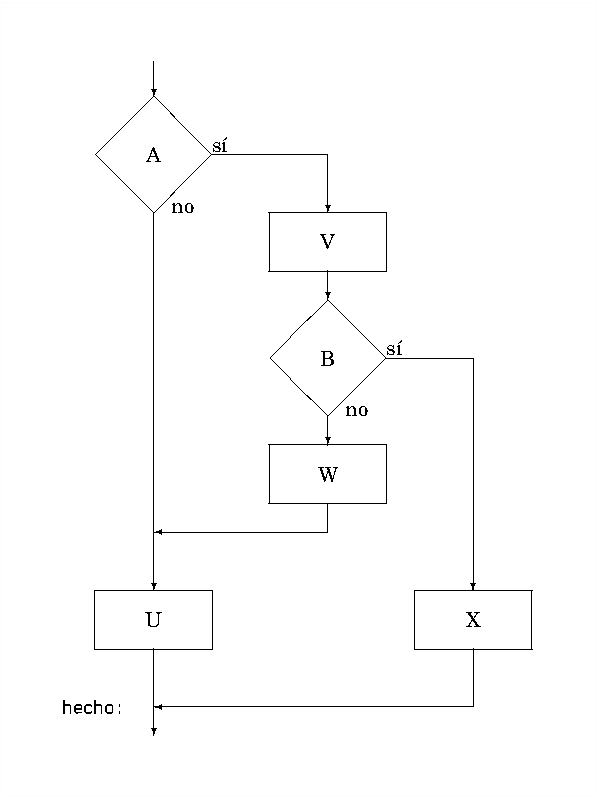
\includegraphics[scale=.8]{diagrama}
\end{center}
\end{minipage}
\hfill
\begin{minipage}{.3\linewidth}
\begin{center}
\NoCaptionOfAlgo
\begin{algorithm}[H]
\caption{con}
\SetKw{goto}{goto}
\DontPrintSemicolon
\If{A}{
  V\;
  \eIf{B}{
  X\;
  \goto \texttt{hecho}\;}{
  W\;}
}
U\;
\texttt{hecho:}
\end{algorithm}
\end{center}
\end{minipage}

¿Podríamos librarnos del «goto» sin duplicar código?

\NoCaptionOfAlgo
\begin{algorithm}[H]
\caption{sin}
\DontPrintSemicolon
\eIf{A}{
  V\;
  \eIf{B}{
    X\;}{
    W\;
    U\;
  }
}{
  U\;
}
\end{algorithm}
\vspace{5mm}

\lipsum[39-41]

\begin{figure}[ht!]
\begin{center}
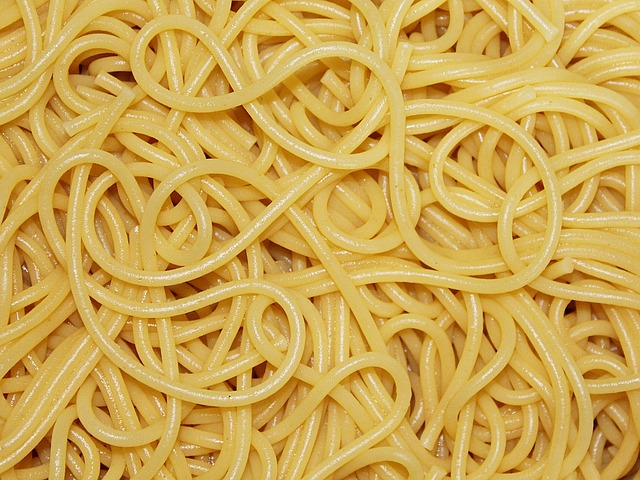
\includegraphics[width=\linewidth]{espaguetis}
\caption{}
\end{center}
\end{figure}

\lipsum[42-43]

\begin{figure}[ht!]
\begin{center}
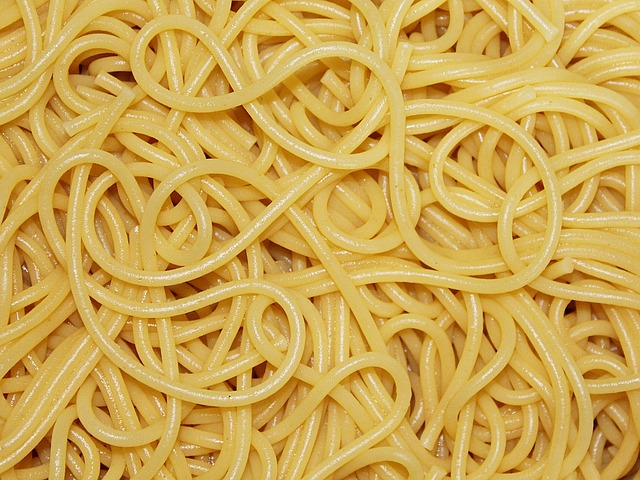
\includegraphics[width=\linewidth]{espaguetis}
\caption*{Sin número}
\end{center}
\end{figure}

\lipsum[45]

\end{comment}
%%%%%%%%%%%%%%%%%%%%%%%%%%%%%%%%%%%%%%%%%%%%%%%%%%%%%%%%%%%%%%%%%%%%%%%%%%%%%%%%%%%%%%%%%%%%%%%%%%%%%%%%%%%%%%%%%%%%%%%%%%%%%%%%%%%%%%%%%%%%%%%%%%%%%%%%%%%%%%%%%%%%%%%%%%%%%%%%%%%%%%%%%%%%%%%%%%%%%%%%%%%%%%%%%%%%%%%%%%%%%%%%%%%%%%%%%%%%%%%%%%%%%%%%%%%%%%%%%%%%%%%%%%%%%%%%%%%%%%%%%%%%%%%%%%%%%%%%%%%%%%%%%%%%%%%%%%%%%%%%%%%%%%%%%%%%%%%%%%%%%%%%%%%%%%%%%%%%%%%%%%%%%%%%%%%%%%%%%%%%%%%%%%%%%%%%%%%%%%%%%%%%%%%%%%%%%%%%%%%%%%%%%%%%%%%%%%%%%%%%%%%%%%%%%%%%%%%%%%%%%%%%%%%%%%%%%%%%%%%%%%%%%%%%%%%%%%%%%%%%%%%%

%VOY A CAMBIAR LA ESTRUCTURA

%Domingo: A few phrases about the structure of this chapter and the goals
This chapter introduces the relationship between probability theory
and Hilbert spaces. We will see that better estimators relate to sampling points that minimize some quantity. The chapter aims to connect all these subject in a rigorous way.
\section{Mean and Variance}
%%%%%%%%Media y varianza 
%(Empezar con second order stereology en CO.IAS.17.Hist.pdf) y 
% seguir con formulas generales??? 
% y formulas para cada problema.
% Domingo: Mejor previous chapter
As it was shown in the previous chapter, estimation problems in Stereology generally make use of the expectation (namely the mean) in order to get a better estimation of the desired quantity. If one wants to know how good of an estimation was obtained, the variance comes into play. However, since the real quantity that we want to estimate is unknown, 
it is necessary to predict the error as well with \textit{variance predictors}, which are usually employed to fulfill the same role as the usual variance.\\

%Domingo: Some reformating, also we did not introduce what is systematic sampling.
We follow the naming convention in Stereology, stating that the mean of a random variable is called a \textit{first order property} and the variance is a \textit{second order property}. We remark that formulas for the variance of %when mean of 
independent estimations are known. However, under systematic sampling the sampled items are correlated to unknown degrees depending on the population pattern, thus the problem is non trivial unless the
%Domingo: Hay que definir que es una random permutation
population is a random permutation (\cite{CO.IAS.17.Hist.pdf}).\\

In probability, we have the following definitions for the mean and the variance of real valued random variables.\\

%Domingo: He añadido la definicion de varianza aqui
\begin{Def}
    Given a sample space $\Omega$, an event space $\sigma$ and a probability function $\mathbb{P}$. If $X$ is a discrete, real valued random variable defined in a probability space $(\Omega, \sigma, \mathbb{P})$, the \textit{mathematical expectation of $X$} and the \textit{variance of $X$} are defined as
    \begin{equation*}
        \mathbb{E}[X]=\sum_n x_n \cdot \mathbb{P}_X[x_n] = \sum_n x_n \cdot \mathbb{P}[X=x_n], \quad Var(X)=\mathbb{E}[(X-\mathbb{E}[X])^2]
    \end{equation*}
    given that the sums exist.
\end{Def}
\vspace{2mm}
\begin{Def}
    Given a sample space $\Omega$, an event space $\sigma$ and a probability function $\mathbb{P}$. If $X$ is a real valued random variable defined in a probability space $(\Omega, \sigma, \mathbb{P})$ such that it's density function $f_X$ exists, the \textit{mathematical expectation of $X$} can be defined as
    \begin{equation*}
        \mathbb{E}[X]=\int_{-\infty}^{\infty} t \cdot f_X(t)\,\mathrm{d}t,
    \end{equation*}
    given that this expression makes sense.
\end{Def}

\vspace{2mm}
Furthermore, a very useful proposition says as follows.\\

\begin{Prop}
    Given a sample space $\Omega$, an event space $\sigma$  and a probability function $\mathbb{P}$. If $X$ is a real valued random variable defined in a probability space $(\Omega,\sigma,\mathbb{P})$ such that $\mathbb{E}[\abs{X}^2]<\infty$, then
    \begin{equation*}
        Var(X)=\mathbb{E}[X^2]-(\mathbb{E}[X])^2
    \end{equation*}
\end{Prop}
\begin{proof} By definition, $Var(X)=\mathbb{E}[(X-\mathbb{E}[X])^2]$. What's more, $$ (X-\mathbb{E}[X])^2 = X^2 + (\mathbb{E}[X])^2 - 2X\mathbb{E}[X]. $$
Given that $\mathbb{E}[X]$ is a real value, applying the expectation we have
\begin{multline*}
    \mathbb{E}[(X-\mathbb{E}[X])^2] = \mathbb{E}[X^2] + \mathbb{E}[(\mathbb{E}[X]^2)] - \mathbb{E}[2X\mathbb{E}[X]] \\ = \mathbb{E}[X^2] + (\mathbb{E}[X])^2 - 2\mathbb{E}[X]\mathbb{E}[X] = \mathbb{E}[X^2] - (\mathbb{E}[X])^2.
\end{multline*}
This finishes the proof.
\end{proof}
\vspace{2mm}

% Mirar cuánto he copiado literal de Cavalieri_basics_R1.pdf xxxxxxxxxxxxxxxxxxxxxxxxxxxxxxxxxxxxxxxxxxxxxxxxxxxxxxxxxxxxxxxxxxxxxxxxxxxxxxxxxxxxxxxxxxxxxxxxxxxxxxxxxxxxxxxxxxxxxxxxxxxxxxxxxxxxxxxxxxxxxxxxxxxxxxxxxxxxxxxxxxxxxxxxxxxxxxxxxxxxxxxxxxxxxxxxxxxxxxxxxxxxxxxxxxxxxxxxxxxxxxxxxxxxxxxxxxxxxxxxxxxxxxxxxxxxxxxxxxxxxxxxxx

%Reescribir con N en vez de T (hecho)
Regarding the error variance estimator, we will now show how to obtain one for the 1-dimensional case. Let $f$ be a predictor function such that it is periodic in $[0,1)$  %Domingo: Hay que cambiar que la funcion tenga soporte acotado por ser periodica.
and define the \textit{covariogram} as
\begin{equation} \label{eqCovariograma}
    g(h) := \int_0^1 f(x) \cdot f(x+h) \,\mathrm{d}x.
\end{equation}
This concept will be of utter importance, so first lets give some basic properties.\\

\begin{Prop}
    If $f$ is a periodic function in $[0,1)$ and $g$ is its covariogram, then the following properties apply:
    \begin{enumerate}
        \item $g$ is symmetric about $h=0$, namely: $g(h) = g(-h)$
        \item $\abs{g(h)} \leq g(0)$ (\textit{i.e.} $\sup_{h}{g(h)} = g(0)$)
        \item $\int_0^1 g(h) \,\mathrm{d}h = \Bigg\{ \int_0^1 f(x) \,\mathrm{d}x \Bigg\}^2 =: V^2$
    \end{enumerate}
\end{Prop}
\begin{proof} 
%Domingo: Asi se veia mal
We start by proving the first item
$$ g(-h) = \int_0^1 f(x) \cdot f(x-h) \,\mathrm{d}x =\{ y=x-h; dy=dx \}= \int_0^1 f(y+h) \cdot f(y) \,\mathrm{d}y = g(h).$$
For the second item
\begin{multline*}
        0 \leq \int_0^1 [ f(x+h) - f(x) ]^2 \,\mathrm{d}x = \int_0^1 f^2(x+h) \,\mathrm{d}x \hspace{1mm} + \int_0^1 f^2(x) \,\mathrm{d}x \hspace{1mm} - 2\cdot \int_0^1 f(x) \cdot f(x+h) \,\mathrm{d}x \\
        = g(0) + g(0) -2\cdot g(h)
    \end{multline*} 
For the last item, 
$$ \int_0^1 \,\mathrm{d}h \int_0^1 f(x) \cdot f(x+h) \,\mathrm{d}x = \int_0^1 f(x) \,\mathrm{d}x \int_0^1 f(x+h) \,\mathrm{d}h = \Bigg\{ \int_0^1 f(x) \,\mathrm{d}x \Bigg\}^2.$$
This finishes the proof.
%Domingo: Una cosa, las ecuaciones se puntuan con punto final.
\end{proof}

\vspace{2mm}

\textbf{Note:} We remark that if $f$ is integrable, then its covariogram is derivable. This will be important when considering the Hilbert space of functions defined later in this chapter.\\%Pregunta??????

%Domingo: Lo he escrito a toda prisa. Espero que este bien
We apply this to design an estimator for the following parameter of interest:
\begin{equation*}
    V = \int_0^1 f(x) \mathrm{d}x,
\end{equation*}
where $f$ is a periodic function, with period $1$.
Lets imagine that we take observations at $z+j/N$ with $j=0,1,2,\ldots, N-1$. An estimator for $V$ reads
\begin{equation*}
    \widehat{V} = \frac{1}{N} \cdot \sum_{j=0}^{N-1} f\left(z+\frac{j}{N}\right) \equiv v(z)
\end{equation*}
which is a periodic function of $z$ with period $1/N$, thus it suffices to consider $z\in (0,1/N)$. As a result, assuming $z \sim U(0,1/N)$ we have
\begin{equation*}
    \mathbb{E}[v(z)] = \int_0^{1/N} \frac{\,\mathrm{d}z}{1/N} \cdot \frac{1}{N}\cdot \sum_j f(z+j/N) = \sum_j \int_0^{1/N} f(z+j/N) \,\mathrm{d}z = \sum_j V_j = V,
\end{equation*}
that is, $v(z)$ is an UE of $V$.\\

Now, by definition,
\begin{equation*}
    Var(v(z)) = \frac{1}{1/N} \int_0^{1/N} v^2(z) \,\mathrm{d}z - V^2 = N \int_0^{1/N} v^2(z) \,\mathrm{d}z - V^2
\end{equation*}
Since $v(z)$ is periodic of period $1/N$, we can write it as a \textit{Fourier series},
\begin{equation*}
    v(z) = \sum_{k=-\infty}^{\infty} c_k \cdot \exp{2\pi i k zN},
\end{equation*}
where 
\begin{equation*}
    c_k = 
    \begin{cases}
         N \int_0^{1/N} v(z) \cdot \exp{(-2\pi i k z N)} \,\mathrm{d}z& (k>0)\\
         N \int_0^{1/N} v(z) \cdot \exp{(2\pi i k z N)} \,\mathrm{d}z& (k<0).
    \end{cases}
\end{equation*}
\vspace{2mm}
%Domingo: Tendriamos que mirar todos los sitios donde has utilizado \exp, no me gusta como queda. Quizás \renewcommand{\exp}[1]{e^{#1}}
Substituting $v(z)$, for $k>0$ we can write
\begin{equation*}
    c_k = N \int_0^{1/N} \frac{1}{N} \cdot \sum_{j=0}^{N-1} f(z+j/N) \cdot \exp{(-2\pi i k z N)} \, \mathrm{d}z = \int_{0}^{1} f(z) \cdot \exp{(-2\pi i k z N)} \,\mathrm{d}z
\end{equation*}
and the conjugate for $k<0$.\\

Using \textit{Parseval's theorem} and $v(z)$'s periodicity we get
\begin{equation*}
    N \int_0^{1/N} v^2(z) \,\mathrm{d}z = \sum_{k=-\infty}^{\infty} c_k \overline{c_k},
\end{equation*}
therefore
\begin{equation*}
    Var(v(z)) = \sum_{k=-\infty}^{\infty} c_k \overline{c_k} - \int_{0}^{1} g(h) \,\mathrm{d}h,
\end{equation*}
where $\overline{c_k}$ is the conjugate of $c_k$.\\

% Domingo  : Los limites son entre 0 y 1, no entre infinito y menos infinitos.
We introduce the following notation
\begin{equation*}
    F(u) := \int_{0}^{1} f(z) \cdot \exp{(-2\pi i u z)} \,\mathrm{d}z,
\end{equation*}
then
\begin{equation*}
    Var(v(z)) = \sum_{k=-\infty}^{\infty} F\left( k N \right) \overline{F}\left( k N \right) - \int_{0}^{1} g(h) \,\mathrm{d}h
\end{equation*}
where $\overline{F}(\cdot)$ is the conjugate of $F(\cdot)$.\\

Consider now the transform of $g(h)$, namely
\begin{multline*}
    G(u) := \int_{0}^{1} g(h) \cdot \exp{(-2\pi i u h)} \,\mathrm{d}h = \int_{0}^{1} f(x) \,\mathrm{d}x \int_{0}^{1} f(x+h) \cdot \exp{(-2\pi i u h)} \,\mathrm{d}h \\
    = \int_{0}^{1} f(x) \,\mathrm{d}x \int_{0}^{1} f(r) \cdot \exp{(-2\pi i u (r-x))} \,\mathrm{d}x = F(u) \cdot \overline{F}(u),
\end{multline*}
then the Fourier coefficients of the Variance have to be symmetric, giving,
\begin{equation*}
    Var(v(z)) = \sum_{-\infty}^{\infty} G\left( k N \right) - G(0) = 2\cdot \sum_{k=1}^{\infty} G\left( k N \right).
\end{equation*}
% Domingo: He escrito esto a toda leche.
In order to have a predictor, we are going to model the variance and suppose that the covariogram can be approximated by a polynomial, namely
\begin{equation*}
    g(h) := \sum_{j=0}^{r} a_j \cdot \abs{h}^j.
\end{equation*}
We substitute the model for the covariogram and calculate the Fourier coefficients: 
%Domingo: BUFFF, ahora me cambia lo de la gamma function. Lo cambio pero 
\begin{equation*}
    G(u) = 2\cdot \int_0^{1} \bigg( \sum_{j=0}^r a_j \cdot h^j \bigg) \cdot \exp{(-2\pi i u h)} \,\mathrm{d}h = 2\cdot \sum_{j=0}^r a_j \int_{0}^{1} h^j \cdot \exp{(-2\pi i u h)} \,\mathrm{d}h.
\end{equation*}
Because we only need real value of the variance, 
that is, the real part of $G(u)$, we define
\begin{equation*}
    \Gamma_{inc} (m) := \int_0^{1} y^{m-1} \cdot \exp{-y} \,\mathrm{d}y \approx \Gamma (m),
\end{equation*}
thus, taking $y=2\pi i u h$ we get
\begin{equation*}
    \int_{0}^{1} h^j \cdot \exp{(-2\pi i u h)} \,\mathrm{d}h = \frac{1}{(2\pi i u)^{j+1}} \int_0^{1} y^j \cdot \exp{(-y)} \,\mathrm{d}y = \frac{\Gamma (j+1)}{(2\pi i u)^{j+1}},
\end{equation*}
and because we want the real part, we only want the terms given by odd $j$, namely $j=2p-1$, $p=1,2,...$ . In consequence,
\begin{equation*}
    Var(v(z)) = 2\cdot \sum_{k=1}^{\infty} Re\left[G\left( k N \right)\right] = 2\cdot \sum_{p=1}^j a_{2p-1} \cdot \frac{1}{N^{2p}} \cdot \Bigg\{ 2\cdot \frac{\Gamma (2p)}{(-1)^p \cdot (2\pi)^{2p}} \cdot \sum_{k=1}^{\infty} \frac{1}{k^{2p}} \Bigg\}
\end{equation*}

Furthermore, since the \textit{Bernoulli number} $B_{2p} \equiv B_{2p}(0)$ can be expressed
\begin{equation*}
    B_{2p}(0) = \frac{(-1)^{p-1} \cdot 2\Gamma (2p+1)}{(2\pi)^{2p}} \cdot \sum_{k=1}^{\infty} \frac{1}{k^{2p}},
\end{equation*}
we can rewrite the variance as
\begin{equation*}
    Var(v(z)) = -\sum_{p=1}^{\lfloor \frac{r+1}{2} \rfloor} a_{2p-1} \cdot \frac{B_{2p}}{p \cdot N^{2p}} = -a_1  \frac{B_2}{N^{2}} -  a_3  \frac{B_4}{2 \cdot N^{4}} - ...
\end{equation*}

Considering that $a_1 = g'(0)$ under the polynomial model and that $B_2 = 1/6$, we can approximate the variance as follows,
\begin{equation*}
    Var(v(z)) \approx -  \frac{g'(0)}{6N^{2}}.
\end{equation*}

Finally, lets fit the parable $g(h) = a_0 + a_1 \cdot h + a_2 \cdot h^2$ through the sample points $\{ (j/N,\widehat{g}(j/N)), \hspace{1mm} j=0,1,2 \}$, where


\begin{equation*}
    \widehat{g}(j/N) = \frac{1}{N}\cdot \sum_{r=1}^{S} f_r \cdot f_{r+j}
\end{equation*}
with $S$ the total number of sections and $f_r$ the \textit{r}-th section area observed at the \textit{r}-th abscissa. More briefly, write
\begin{equation*}
    g_0 \equiv \sum f_i^2,\quad 
    g_1 \equiv \sum f_i \cdot f_{i+1},\quad
\mathrm{ and} \
    g_2 \equiv \sum f_i \cdot f_{i+2},
\end{equation*}
where $f_i \equiv f(z+i/N)$ and thus $\widehat{g}(j/N) \equiv \frac{1}{N}\cdot g_j$.
Then we have
\begin{equation*}
    \frac{1}{N} \cdot g_0 = a_0,\quad
    \frac{1}{N} \cdot g_1 = a_0 + a_1 \cdot \frac{1}{N} + a_2 \cdot \frac{1}{N^2},\quad 
    \frac{1}{N} \cdot g_2 = a_0 + a_1 \cdot \frac{2}{N} + a_2 \cdot \left(\frac{2}{N}\right)^2
\end{equation*}
from which we get
\begin{equation*}
    a_1 = \frac{4g_1 - g_2 - 3g_0}{2}.
\end{equation*}
\vspace{2mm}

Therefore, we can get the following variance estimator,
\begin{equation*}
    \widehat{Var(v(z))} \approx - \frac{a_1}{6N^2} = \frac{3g_0 + g_2 - 4g_1}{12} \cdot \frac{1}{N^2}
\end{equation*}

\vspace{2mm}

This is the general method to approximate the variance. Next, we will present the error variance estimators that have been developed for the two estimation procedures that will be used in this work. The method to discover them follows the same principles but the proofs are more involved due to the number of variables.
After that we will explain how the expectations are calculated.\\



\section{Variance prediction formula of particle number estimation in the plane with a test system of quadrats}

Consider $Y\subset \mathbb{R}^2$ a bounded and finite set of $N\equiv N(Y)$ particles. We want to estimate $N$ using a test system of quadrats $\Lambda_x$ whose fundamental tile $J_0$ is a square with side length $T$ and whose fundamental probe $T_0$ is a square quadrat with side length $0<t\leq T$. Let $Q$ represent the number of particles captured by $\Lambda_x$, $x\sim UR(J_0)$. Since $Y$ contains point particles, $Q$ is the total number of particles within the quadrats, otherwise, the particles should be captured using unbiased sampling rules such as the \textit{forbidden line rule}.\\

As it was shown in the first chapter, an UE for $N$ is given by
\begin{equation*}
    \widehat{N} = \frac{a}{a_0} \cdot Q = \frac{T^2}{t^2} \cdot Q
\end{equation*}
In an effort to interpret the error variance predictor for $\widehat{N}$, the test system is regarded as a two stage sample:
\begin{itemize}
    \item \textit{First stage sample:} It consists of a set of $n$ Cavalieri stripes of thickness $t$ and period $T$ encompassing the particle population $Y$.
    \item \textit{Second stage sample:} It consists of another set of Cavalieri stripes with the same period and thickness but perpendicular to the other one.
\end{itemize}
Using this two stage sample, we get something similar to $\Lambda_x$ providing new data such as $Q_{oi}$ and $Q_{ei}$, namely the number of particles captured by the odd and even quadrats within the \textit{i}th stripe respectively. This means that $Q_i=Q_{oi}+Q_{ei}$ is the number of particles captured by all quadrats within the \textit{i}-th stripe, therefore $Q=\sum_{i=1}^n Q_i$. As a result, a variance predictor for $\widehat{N}$ can be obtained as follows,%Importante lo de []
\begin{equation*}
    Var(\widehat{N}) = \frac{\alpha(0,\tau)}{\tau^4}\cdot [3(C_0-\widehat{\nu}_n) - 4C_1 + C_2] + \frac{\widehat{\nu}_n}{\tau^4}, \hspace{2mm} n\geq 3
\end{equation*}
where $\tau = t/T \in (0,1]$,
\begin{equation*}
    C_k = \sum_{i=1}^{n-k}Q_i Q_{i+k}, \hspace{2mm} k=0,1,2,
\end{equation*}
\begin{equation*}
    \widehat{\nu}_n = \sum_{i=1}^n Var(Q_i) = \frac{(1-\tau)^2}{3-2\tau} \cdot \sum_{i=1}^n (Q_{oi}-Q_{ei})^2
\end{equation*}
and
\begin{equation*}
    \alpha(0,\tau) = \frac{1}{6}\cdot \frac{(1-\tau)^2}{2-\tau}.
\end{equation*}
\textbf{Note:} This variance predictor must first be evaluated for a given direction of the stripes, and then for the perpendicular direction. The \textit{real variance predictor} is the average of both results (\cite{SterThAppl-2022-07-21.pdf}).


\section{Variance prediction formula of curve length in the plane with a Buffon-Steinhaus test system}

Consider $Y \subset \mathbb{R}^2$ a bounded, piecewise smooth curve with finite length $B>0$. We want to estimate $B$ using the Buffon-Steinhaus test system, namely a square grid whose fundamental tile $J_0$ is a square with side length $T>0$. Similarly to what's been done in the last section, consider the square grid as two different sets of Cavalieri lines (namely \textit{set 1} and \textit{set 2}) of period $T$, making angles $\omega$ and $\omega + \pi/2$ with a fixed axis, where $\omega \sim IR[0,\pi/2)$. Now, for the set \textit{i}, let 
\begin{equation*}
    \{ I_{i1}, I_{i2}, ..., I_{in_i} \}, \hspace{2mm} i=1,2,
\end{equation*}
denote the number of intersections determined by each one of the $n_i$ Cavalieri lines hitting the curve. As one would expect,
\begin{equation*}
    I_i = \sum_{j=1}^{n_i} I_{ij}, \hspace{2mm} i=1,2,
\end{equation*}
denotes the number of intersections determined by the set \textit{i} hitting the curve. Whereby, an UE for B is given by
\begin{equation*}
    \widehat{B} = \frac{\pi}{4} \cdot T \cdot (I_1+I_2).
\end{equation*}
An equivalent design is obtained if the curve is equipped with an associated vector $(x,\omega)$, with $x\sim UR(J_0)$ and $\omega \sim IR[0,2\pi)$.\\

That being said, a variance predictor for $\widehat{B}$ can be obtained as follows,
\begin{equation*}
    Var(\widehat{B}) = \frac{\pi^2}{96} \cdot [(\widehat{l_1}-\widehat{l_2})^2-\widehat{\nu}_2] + \frac{\pi^2}{16}\cdot \widehat{\nu}_2,
\end{equation*}
where
\begin{equation*}
    \widehat{l_i} = T \cdot I_i,
\end{equation*}
\begin{equation*}
    \widehat{\nu}_2 = \sum_{i=1}^2 Var(\widehat{l_i}|l_i),
\end{equation*}
\begin{equation*}
    Var(\widehat{l_i}|l_i) = \frac{T^2}{12} \cdot (3C_{0i} - 4C_{1i} + C_{2i}), \hspace{2mm} n_i\geq 3,
\end{equation*}
\begin{equation*}
    Var(\widehat{l_i}|l_i) = \frac{T^2}{6} \cdot (C_{0i} - C_{1i}), \hspace{2mm} n_i = 2,
\end{equation*}
\begin{equation*}
    C_{ki} = \sum_{i=1}^{n_i - k} I_{ij} I_{i,j+k}, \hspace{2mm} k=0,1,...,n_i-1, \hspace{2mm} i=1,2.
\end{equation*}
The results and discussions for these two latter sections can be found in \citep{SterThAppl-2022-07-21.pdf}.

\section{Quasi-Monte Carlo Integration (QMC Integration)}
%Forma de calcular las esperanzas a partir de sumas en vez de integrales. También objetivo de lo que se pretende (mejorar la eficiencia).
%%%%%%%%%%%%%%%%%%%%%%%%%%%%%%%%%%%%%%%%%%%%%%%%%%%%%%%%%%%%%%%
% Samplings points in quasi-montecarlo integration method. (Hinrich.pdf) 
% Spaces of functions (https://en.wikipedia.org/wiki/Reproducing_kernel_Hilbert_space). 
% Error depending 

One problem that has to be dealt with in order to compute the target measure estimate, is the numerical integration of multivariate functions. This problem arises because of the need to obtain the expectation, in this case for the number of intersections in both estimation problems.\\

To simplify things, lets normalize the integration domain to be the compact unit cube $[0,1]^d$, that is,
\begin{equation*}
    \int_{[0,1]^d} f(\textbf{x})\,\mathrm{d}\textbf{x} = \int_0^1 \cdot \cdot \cdot \int_0^1 f(x_1,...,x_d)\,\mathrm{d}x_1\ldots\mathrm{d}x_d
\end{equation*}
The goal is to approximate these integrals using \textit{QMC rules} with fixed integration nodes $\textbf{x}_0,...,\textbf{x}_{N-1} \in [0,1)^d$, namely
\begin{equation} \label{QMC}
    \int_{[0,1]^d} f(\textbf{x})\,\mathrm{d}\textbf{x} \approx \mathcal{Q}_{N,d}(f) := \frac{1}{N} \sum_{n=0}^{N-1} f(\textbf{x}_n).
\end{equation}
\vspace{2mm}

The crux of this method is the choice of underlying nodes. What's more, we also need some global information on the functions to be integrated, since one can find two functions $f,g : [0,1]^d \longrightarrow \mathbb{R}$ such that $f(\textbf{x}_n) = g(\textbf{x}_n) \hspace{2mm} \forall n=0,1,...,N-1$, but $\int_{[0,1]^d} f(\textbf{x})\,\mathrm{d}\textbf{x} - \int_{[0,1]^d} g(\textbf{x})\,\mathrm{d}\textbf{x}$ can be any number. So as to avoid this problem, function classes with certain smoothness properties are considered.\\

Lets start with \textit{univariate QMC integration}, namely QMC integration of univariate real valued functions $f:[0,1] \longrightarrow \mathbb{R}$ with continuous first derivative on $[0,1]$. From the \textit{fundamental theorem of calculus} we have
\begin{equation*}
    f(x) = f(1) - \int_x^1 f'(y)\,\mathrm{d}y, \hspace{2mm} \forall x \in [0,1].
\end{equation*}
For the error of a QMC rule based on sample nodes $\mathcal{P}=\{ x_0,...,x_{N-1} \} \subset [0,1)$ we then get
\begin{multline*}
    e(f,\mathcal{P}) = \int_0^1 f(x)\,\mathrm{d}x - \frac{1}{N} \sum_{n=0}^{N-1} f(x_n) = -\int_0^1 \int_x^1 f'(y)\,\mathrm{d}y \,\mathrm{d}x + \frac{1}{N} \sum_{n=0}^{N-1} \int_{x_n}^1 f'(y) \,\mathrm{d}y \\
    = -\int_0^1 \int_0^y f'(y)\,\mathrm{d}x \,\mathrm{d}y + \int_0^1 \frac{1}{N} \sum_{n=0}^{N-1} 1_{(x_n,1]}(y) f'(y) \,\mathrm{d}y = \int_0^1 f'(y) \Bigg[\frac{1}{N} \sum_{n=0}^{N-1} 1_{(x_n,1]}(y) - y\Bigg] \,\mathrm{d}y
\end{multline*}
Since the number of indices $n\in \{ 0,...,N-1 \}$ for which $x_n \in [0,y)$ is
\begin{equation*}
    \sum_{n=0}^{N-1} 1_{(x_n,1]}(y) = \sum_{n=0}^{N-1} 1_{(0,y]}(x_n)
\end{equation*}
we find that
\begin{equation*}
    \frac{1}{N} \sum_{n=0}^{N-1} 1_{(x_n,1]}(y) - y = \Delta_{\mathcal{P},N}(y),
\end{equation*}
that is, the local discrepancy of $\mathcal{P}$ in $y$. Therefore,
\begin{equation*}
    e(f,\mathcal{P}) = \int_0^1 f'(y)\Delta_{\mathcal{P},N}(y)\,\mathrm{d}y.
\end{equation*}

Taking the absolute value and applying the \textit{triangle inequality for integrals} and the \textit{Hölder inequality} we get
\begin{equation*}
    \abs{e(f,\mathcal{P})} \leq \int_0^1 \abs{f'(y)} \abs{\Delta_{\mathcal{P},N}(y)} \,\mathrm{d}y \leq \left( \int_0^1 \abs{f'(y)}^r \,\mathrm{d}y \right)^{1/r} \left(  \int_0^1 \abs{\Delta_{\mathcal{P},N}(y)}^s \,\mathrm{d}y \right)^{1/s} \\
    = \norm{f'}_{L_r} \norm{\Delta_{\mathcal{P},N}}_{L_s},
\end{equation*}
where $r,s \in [0,\infty]$ such that $\frac{1}{r} + \frac{1}{s} = 1$. For QMC integration of functions $f$ for which $\norm{f'}_{L_r} < \infty$, sample nodes $\mathcal{P}$ with low $L_s$ discrepancy $L_{s,N}(\mathcal{P}) = \norm{\Delta_{\mathcal{P},N}}_{L_s}$ should be chosen.\\

\textbf{Note:}
In order to develop a similar theory for multivariate functions, the notion of \textit{reproducing kernel Hilbert space} will be used.
For an integrable function $f : [0,1]^d \longrightarrow \mathbb{C}$ and a point set $\mathcal{P} = \{\textbf{x}_0,...,\textbf{x}_N-1\} \subset [0,1)^d$, the notation:
\begin{equation*}
    e(f,\mathcal{P}) = \int_{[0,1]^d} f(\textbf{x}) \,\mathrm{d}\textbf{x} - \frac{1}{N} \sum_{n=1}^{N-1} f(\textbf{x}_n),
\end{equation*}
will be used in analogy to the univariate case. What's more, the inner product in a \textit{Hilbert Space} $\mathcal{H}$ will be denoted by $\langle \cdot,\cdot \rangle$ and the corresponding norm will be denoted by $\norm{\cdot} = \langle \cdot,\cdot \rangle^{1/2}$.\\


Now lets give some useful definitions used with Hilbert spaces in order to develop a similar theory for multivariate functions.\\

\begin{Def}
    The \textit{worst-case error} of a QMC rule based on a point set $\mathcal{P} = \{\textbf{x}_0,...,\textbf{x}_N-1\} \subset [0,1)^d$ in a Hilbert space $\mathcal{H}$ of integrable functions on $[0,1]^d$ is defined as
    \begin{equation*}
        e(\mathcal{H},\mathcal{P}) = \underset{f \in \mathcal{H}, \norm{f}\leq 1}{\text{sup}} \abs{e(f,\mathcal{P})}.
    \end{equation*}
\end{Def}

\vspace{2mm}
Also, the notion of \textit{reproducing kernel} will be important for our purposes.\\

\begin{Def}
    A Hilbert space $\mathcal{H}$ of functions on $[0,1]^d$ is a \textit{reproducing kernel Hilbert space} on $[0,1]^d$ if there exists a function $K : [0,1]^d \times [0,1]^d \longrightarrow \mathbb{C}$ such that
    \begin{itemize}
        \item[K1:]\label{K1} $K(\cdot,\textbf{y}) \in \mathcal{H} \hspace{2mm} \forall \textbf{y} \in [0,1]^d$ 
        \item[K2:]\label{K2} $\langle f,K(\cdot,\textbf{y}) \rangle = f(\textbf{y}) \hspace{2mm} \forall \textbf{y} \in [0,1]^d, \hspace{1mm} \forall f\in \mathcal{H}$.
    \end{itemize}
    The function $K$ is the \textit{reproducing kernel} of $\mathcal{H}$.\\
\end{Def}

\textbf{Note:} the reproducing kernel $K$ has been considered as a function of the first variable, denoted by $\cdot$, thus, in $\langle f,K(\cdot,\textbf{y}) \rangle$ the inner product is applied with respect to the first variable of $K$.\\


Furthermore, reproducing kernels have the following properties.\\

\begin{Corollary}
    A function satisfying K1 and K2 is symmetric, uniquely defined and positive semi-definite, that is,
    \begin{itemize} 
        \item[K3:]\label{K3} $K(\textbf{x},\textbf{y}) = \overline{K(\textbf{y},\textbf{x})} \hspace{2mm} \forall \textbf{x},\textbf{y} \in [0,1]^d$ (symmetry) 
        \item[K4:]\label{K4} If a function $\Tilde{K}$ satisfies K1 and K2, then $\Tilde{K} = K$ (uniqueness)
        \item[K5:]\label{K5} For any $a_0,...,a_{N-1} \in \mathbb{C}$ and $\textbf{x}_0,...,\textbf{x}_{N-1} \in [0,1]^d$, we have $\sum_{m,n=0}^{N-1} \Tilde{a}_m a_n K(\textbf{x}_m,\textbf{x}_n) \geq 0$ (positive semi-definiteness) 
    \end{itemize}
\end{Corollary}
\begin{proof} K3: $K(\textbf{x},\textbf{y}) = \langle K(\cdot,\textbf{y}),K(\cdot,\textbf{x}) \rangle = \overline{\langle K(\cdot,\textbf{x}),K(\cdot,\textbf{y}) \rangle} = \overline{K(\textbf{y},\textbf{x})} $.\\
K4: $\Tilde{K}(\textbf{x},\textbf{y}) = \langle \Tilde{K}(\cdot,\textbf{y}),K(\cdot,\textbf{x}) \rangle = \overline{\langle K(\cdot,\textbf{x}),\Tilde{K}(\cdot,\textbf{y}) \rangle} = \overline{K(\textbf{y},\textbf{x}) = K(\textbf{x},\textbf{y})}$.\\
K5: 
\begin{multline*}
    \sum_{m,n=0}^{N-1} \Tilde{a}_m a_n K(\textbf{x}_m,\textbf{x}_n) = \sum_{m,n=0}^{N-1} \Tilde{a}_m a_n \langle K(\cdot,\textbf{x}_n),K(\cdot,\textbf{x}_m) \rangle = \langle \sum_{n=0}^{N-1} a_n K(\cdot,\textbf{x}_n),\sum_{m=0}^{N-1} a_m K(\cdot,\textbf{x}_m) \rangle \\
    = \begin{Vmatrix} \sum_{m=0}^{N-1} a_m K(\cdot,\textbf{x}_m) \end{Vmatrix}^2 \geq 0.
\end{multline*} 

This concludes the proof.
\end{proof}

\vspace{2mm}
Additionally, a function $K$ satisfying K3 and K5 uniquely determines a Hilbert space of functions  for which K1, K2 and K4 hold. Whereby, it makes sense to speak of a reproducing kernel without specifying the corresponding Hilbert space.\\

That being said, let $\mathcal{H}$ be a Hilbert space of integrable functions $f : [0,1]^d \longrightarrow \mathbb{C}$ equipped with inner product $\langle \cdot,\cdot \rangle$ and corresponding norm $\norm{\cdot} = \langle \cdot,\cdot \rangle^{1/2}$.\\

\begin{Def}
    A linear functional $T$ on $\mathcal{H}$ is \textit{bounded} if there exists $M<\infty$ such that $\abs{T(f)}\leq M$ for all $f$ with $\norm{f}\leq 1$.
\end{Def}

\vspace{2mm}
Also, it is known that linear functionals boundedness is equivalent to continuity.\\

Lets consider $e(\mathcal{H},\mathcal{P})$ (\textit{i.e.} the worst-case error of a QMC rule based on a point set $\mathcal{P}\subset [0,1)^d$ in $\mathcal{H}$). It's not clear if $e(\mathcal{H},\mathcal{P})$ is finite, that is to say, if the linear functional $e(\cdot,\mathcal{P})$ is continuous. However, conditions exist such that this is the case.\\

Let $T_y$ be the linear functional that evaluates $f\in \mathcal{H}$ at $\textbf{y}\in [0,1]^d$, namely
\begin{equation*}
    T_y(f) = f(\textbf{y}) \hspace{2mm} \text{for } f\in \mathcal{H}.
\end{equation*}
$T_y$ is called the \textit{evaluation functional} in $y$. It turns out that if $T_y$ is continuous $\forall \textbf{y} \in [0,1]^d$, then so is every QMC rule. What's more, continuity of the evaluation functional is equivalent to the existence of a reproducing kernel.\\

\begin{Th}
    Let $\mathcal{H}$ be a Hilbert space of functions on $[0,1]^d$. $\mathcal{H}$ is a reproducing kernel Hilbert space on $[0,1]^d$ if and only if the evaluation functionals $$ T_y(f) = f(\textbf{y}) \hspace{2mm} \text{for } f \in \mathcal{H}, \textbf{y} \in [0,1]^d $$ are continuous.
\end{Th}
\begin{proof} $\Leftarrow)$ We assume that the evaluation functionals are continuous, therefore, the \textit{Fréchet-Riesz Representation Theorem} guarantees that, for every $\textbf{y}$, a uniquely determined function $k_y \in \mathcal{H}$ exists such that $$ T_y(f) = \langle f,k_y \rangle \hspace{2mm} \forall f \in \mathcal{H}.$$ Defining $K(\textbf{x},\textbf{y}) := k_y(\textbf{x})$ for $\textbf{x},\textbf{y} \in [0,1]^d$, properties K1 and K2 are satisfied by $K$, thus $\mathcal{H}$ is a reproducing kernel Hilbert space whose reproducing kernel is $K$.\\ 

$\Rightarrow)$ Assume $K$ is a reproducing kernel for $\mathcal{H}$ and let $\textbf{y} \in [0,1]^d$. Using the Cauchy-Schwarz inequality, we get $$ \abs{T_y(f)} = \abs{f(\textbf{y})} = \abs{\langle f,K(\cdot,\textbf{y}) \rangle} \leq \norm{f} \norm{K(\cdot,\textbf{y})} \hspace{2mm} \forall f \in \mathcal{H}.$$
Now, using K2 we have $\norm{K(\cdot,\textbf{y})}^2 = \langle K(\cdot,\textbf{y}),K(\cdot,\textbf{y}) \rangle = K(\textbf{y},\textbf{y})$, whereby $\abs{T_y(f)}\leq M := \sqrt{K(\textbf{y},\textbf{y})}$ for every $f$ with $\norm{f}\leq 1$. This means that $T_y$ is continuous, which concludes the proof. %Pregunta????
\end{proof}

\vspace{2mm}
Continuing with the situation above, lets consider the integration functional $I(f) = \int_{[0,1]^d} f(\textbf{x})\,\mathrm{d}\textbf{x}$. If $\mathcal{H}$ has a reproducing kernel $K$, then for any $f \in \mathcal{H}$ with $\norm{f}\leq 1$ we have
\begin{equation*}
    \abs{\int_{[0,1]^d} f(\textbf{y}) \,\mathrm{d}\textbf{y}} = \abs{\int_{[0,1]^d} T_y(f) \,\mathrm{d}\textbf{y}} \leq \int_{[0,1]^d} \abs{T_y(f)} \,\mathrm{d}\textbf{y} \leq \int_{[0,1]^d} \sqrt{K(\textbf{y},\textbf{y})} \,\mathrm{d}\textbf{y}.
\end{equation*}
Therefore, if the reproducing kernel $K$ satisfies
\begin{itemize}
    \item[$\textbf{C}$:] $\int_{[0,1]^d} \sqrt{K(\textbf{y},\textbf{y})} \,\mathrm{d}\textbf{y} < \infty$,
\end{itemize}
then the integration functional $I$ is continuous.\\

In conclusion, if $\mathcal{H}$ has a reproducing kernel $K$ that satisfies $\textbf{C}$, then function evaluation and integration are continuous linear functionals, and so is $e(\cdot,\mathcal{P})$ for any point set $\mathcal{P}$. What's more, under these conditions $e(\mathcal{H},\mathcal{P})$ is a well-defined finite number.\\

A very important property for the error analysis follows.\\

\begin{Lemma}
    Let $\mathcal{H}$ be a reproducing kernel Hilbert space with reproducing kernel $K$ and inner product $\langle \cdot,\cdot \rangle$. If the mapping
    \begin{equation*}
        I(f) = \int_{[0,1]^d} f(\textbf{y}) \,\mathrm{d}\textbf{y} \hspace{2mm} \text{for } f\in \mathcal{H}
    \end{equation*}
    is a continuous linear functional on $\mathcal{H}$, then
    \begin{equation*}
        \int_{[0,1]^d} \langle f,K(\cdot,\textbf{y}) \rangle \,\mathrm{d}\textbf{y} = \langle f,\int_{[0,1]^d} K(\cdot,\textbf{y}) \,\mathrm{d}\textbf{y} \rangle.
    \end{equation*}
\end{Lemma}
\begin{proof} We assume that $I$ is continuous, therefore, the Fréchet-Riesz representation theorem guarantees the existence of a uniquely determined function $R \in \mathcal{H}$ such that
\begin{equation*}
    \int_{[0,1]^d} f(\textbf{y}) \,\mathrm{d}\textbf{y} = I(f) = \langle f,R \rangle \hspace{2mm} \forall f\in \mathcal{H}.
\end{equation*}
Given that $R\in \mathcal{H}$, we have
\begin{equation*}
    R(\textbf{x}) = \langle R,K(\cdot,\textbf{x}) \rangle = \overline{\langle K(\cdot,\textbf{x}),R \rangle} = \overline{\int_{[0,1]^d} K(\textbf{y},\textbf{x}) \,\mathrm{d}\textbf{y}}.
\end{equation*}
Whereby
\begin{multline*}
    \int_{[0,1]^d} \langle f,K(\cdot,\textbf{y}) \rangle \,\mathrm{d}\textbf{y} = \int_{[0,1]^d} f(\textbf{y}) \,\mathrm{d}\textbf{y} = \langle f,R \rangle = \langle f,\overline{\int_{[0,1]^d} K(\textbf{y},\cdot) \,\mathrm{d}\textbf{y}} \rangle \\
    = \langle f,R \rangle = \langle f,\int_{[0,1]^d} K(\cdot,\textbf{y}) \,\mathrm{d}\textbf{y} \rangle.
\end{multline*}

This concludes the proof.
\end{proof}

\textbf{Note:} From now on, $K$ will be assumed to satisfy the condition \textbf{$C$}.\\

Lets continue the worst-case error analysis. We have
\begin{equation*}
    I(f) = \int_{[0,1]^d} \langle f,K(\cdot,\textbf{y}) \rangle \,\mathrm{d}\textbf{y} = \langle f,\int_{[0,1]^d} K(\cdot,\textbf{y}) \,\mathrm{d}\textbf{y} \rangle.
\end{equation*}
On the other hand, we have
\begin{equation*}
    \mathcal{Q}_{N,d}(f) = \frac{1}{N} \sum_{n=0}^{N-1} f(\textbf{x}_n) = \frac{1}{N} \sum_{n=0}^{N-1} \langle f,K(\cdot,\textbf{x}_n) \rangle = \langle f,\frac{1}{N} \sum_{n=0}^{N-1} K(\cdot,\textbf{x}_n) \rangle.
\end{equation*}
Therefore, the QMC rule $\mathcal{Q}_{N,d}$ in $\mathcal{H}$ has an integration error that can be expressed as an inner product, namely
\begin{equation*}
    e(f,\mathcal{P}) = \langle f,h \rangle,
\end{equation*}
where
\begin{equation*}
    h(\textbf{x}) = \int_{[0,1]^d} K(\textbf{x},\textbf{y}) \,\mathrm{d}\textbf{y} - \frac{1}{N} \sum_{n=0}^{N-1} K(\textbf{x},\textbf{x}_n).
\end{equation*}
The function above is called the \textit{representer} of the integration error. Taking the absolute value and applying the Cauchy-Schwarz inequality, we get
\begin{equation*}
    \abs{e(f,\mathcal{P})} \leq \norm{f} \cdot \norm{h}.
\end{equation*}
What's more, among all functions in the unit ball of $\mathcal{H}$, the normalized representer (\textit{i.e.} $h/\norm{h}$) is the hardest to integrate. Thus, the worst-case error reads
\begin{equation*}
    e(\mathcal{H},\mathcal{P}) = \norm{h}.
\end{equation*}
As a result, the squared worst-case error can be written as
\begin{equation*}
    e^2(\mathcal{H},\mathcal{P}) = \langle h,h \rangle.
\end{equation*}

\vspace{2mm}
Finally, these results derive in the following theorem, which states the maximum integration error in terms of $\mathcal{P}$.\\

\begin{Th}
    Let $\mathcal{H}$ be a reproducing kernel Hilbert space with reproducing kernel $K$ such that condition \textbf{$C$} is satisfied, and let $\mathcal{P} = \{ \textbf{x}_0,...,\textbf{x}_{N-1} \} \subset [0,1)^d$ be a point set with $N$ elements. Then
    \begin{equation} \label{worst-case error original}
        e^2(\mathcal{H},\mathcal{P}) = \int_{[0,1]^d} \int_{[0,1]^d} K(\textbf{x},\textbf{y}) \,\mathrm{d}\textbf{x} \,\mathrm{d}\textbf{y} - \frac{2}{N} \sum_{n=0}^{N-1} \int_{[0,1]^d} K(\textbf{x}_n,\textbf{y}) \,\mathrm{d}\textbf{y} + \frac{1}{N^2} \sum_{n,m=0}^{N-1} K(\textbf{x}_n,\textbf{x}_m)
    \end{equation}
\end{Th}

\vspace{4mm}
On the other hand, there is the problem of choosing the nodes that will be used for the QMC rule. One way of solving this problem is to use what's called a \textit{lattice point set}.\\

\begin{Def}
    Let $d,N \in \mathbb{N}$, $N\geq 2$ and let $\textbf{g}\in \mathbb{Z}^d$. A point set $\mathcal{P}(\textbf{g},N) = \{ \textbf{x}_0,...,\textbf{x}_{N-1} \}$ with 
    \begin{equation*}
        \textbf{x}_n := \Big\{ \frac{n}{N} \textbf{g} \Big\} \hspace{2mm} \forall n=0,1,...,N-1
    \end{equation*}
    is called a lattice point set and $\textbf{g}$ is its \textit{generating vector}.
\end{Def}

\vspace{2mm}
These lattice point sets have the following property,
\begin{equation*}
    \sum_{n=0}^{N-1} \exp{2\pi i n\textbf{h} \cdot \textbf{g} / N} = \Bigg\{ 
    \begin{matrix}
        N & \text{if } \textbf{h} \cdot \textbf{g} \equiv 0 \hspace{2mm} (\text{mod } N)\\
        0 & \text{if } \textbf{h} \cdot \textbf{g} \not\equiv 0 \hspace{2mm} (\text{mod } N),
    \end{matrix}
\end{equation*}
which allow them to get low values for the worst-case error (see eq. \ref{worst-case error original}). In order to do so, it is enough to find a generating vector $\textbf{g} \in \{ 0,...,N-1 \}^d$. Since checking $N^d$ integer vectors is not feasible in practice for big $N$ and $d$ values, an algorithm was developed that makes it able to create the generating vector component-by-component (CBC).\\

\begin{Algorithm} \label{CBC}
     \textbf{(CBC Algorithm).} Let $d,N \in \mathbb{N}$.
     \begin{enumerate}
         \item Choose $g_1 = 1$.
         \item For $k=2,3,...,d$, choose $g_k \in \{ 1,...,N-1 \}$ that minimizes $R_N((g_1,...,g_{k-1},z))$ as a function of $z \in \{ 1,...,N-1 \}$, 
     \end{enumerate}
\end{Algorithm}
where
\begin{equation*}
    R_N(\textbf{g}) := \sum_{\textbf{h}\in C_d^*(N)\cap \mathcal{L(\textbf{g},N)}} \frac{1}{r_1(\textbf{h})},
\end{equation*}
\begin{equation*}
    r_1(\textbf{h}) = \prod_{i=1}^d r_1(h_i),
\end{equation*}
\begin{equation*}
    r_1(h) := \max{\{1,\abs{h}\}},
\end{equation*}
\begin{equation*}
    C_d^*(N) := \left[ \left( -N/2,N/2 \right] \cap \mathbb{Z} \right]^d\setminus\{0\}
\end{equation*}
and
\begin{equation*}
    \mathcal{L}(\textbf{g},N) := \{ \textbf{h} \in \mathbb{Z}^d : \textbf{h} \cdot \textbf{g} \equiv 0 \hspace{2mm} (\text{mod } N) \}
\end{equation*}
is the \textit{dual lattice} of the lattice point set $\mathcal{P}(\textbf{g},N)$ (\cite{Leobacher_Pillichshammer___2013___Introduction_to_Quasi_Montecarlo_Methods.pdf}).\\

Having said that, several QMC constructions exist for which the optimal rate of convergence $\mathcal{O}(N^{-1}\log(N)^{1/2})$ yields asymptotically, but it's yet unknown what the optimal point set is (in the sense that it's a global minimizer of the worst case integration error). However, for small Fibonacci numbers $N$, it is known that the unique minimizer of the QMC worst-case error in the reproducing kernel Hilbert space $H_{mix}^1$ of 1-periodic functions with mixed smoothness is the Fibonacci lattice. What's more, for $N=1,2,3,5,7,8,12,13$ the optimal point sets are integration lattices (\cite{Hinrichs.pdf}).\\



\section{Optimal Point Sets for QMC Integration}
%Básicamente hablar de los puntos de Hinrichs

Let's consider the reproducing kernel Hilbert space $H_{mix}^1$ of 1-periodic functions with mixed smoothness. It's reproducing kernel is a tensor product kernel that reads
\begin{equation*}
    K_{d,\gamma}(\textbf{x},\textbf{y}) := \prod_{i=1}^{d} K_{1,\gamma}(x_i,y_i),
\end{equation*}
where $\textbf{x}=(x_1,...,x_d), \textbf{y}=(y_1,...,y_d)\in [0,1)^d$, 
\begin{equation*}
    K_{1,\gamma}(x,y) = 1 + \gamma k(\abs{x-y}),
\end{equation*}
\begin{equation*}
    k(t) = \frac{1}{2} (t^2 - t + \frac{1}{6})
\end{equation*}
and $\gamma > 0$ is a parameter. \\

As a result, if we consider a point set $\mathcal{P} = \{ \textbf{x}_0,...,\textbf{x}_{N-1} \}$, then minimizing the worst-case error $e(H_{mix}^1,\mathcal{P})$ with respect to the Hilbert space norm corresponding to the reproducing kernel $K_{d,\gamma}$ is equivalent to minimizing the double sum
\begin{equation*}
    G_{\gamma}(\textbf{x}_0,...,\textbf{x}_{N-1}) = \sum_{n,m=0}^{N-1} K_{d,\gamma}(\textbf{x}_n,\textbf{x}_m).
\end{equation*}

It is known that the Fibonacci lattice yields the optimal point configuration for integrating periodic functions, which may suggest that the optimal point configurations are integration lattices or at least lattice point sets, however, that's not always true. Nonetheless, integration lattices are always local minima of $e(H_{mix}^1,\mathcal{P})$. What's more, for small $\gamma$ values the optimal points are always close to a lattice point set, which for $d=2$ gives point sets of the form
\begin{equation*}
    \Bigg\{ \left(\frac{i}{N},\frac{\sigma(i)}{N}\right) : i=0,...,N-1 \Bigg\},
\end{equation*}
where $\sigma$ is a permutation of $\{ 0,1,...,N-1 \}$.\\


In order to obtain these optimal point sets various considerations have to be contemplated. First, lets consider univariate 1-periodic functions $f : \mathbb{R} \longrightarrow \mathbb{R}$ given by their values on the torus $\mathbb{T} = [0,1)$.\\

\begin{Def}
    Let $k\in \mathbb{Z}$, the \textit{$k$-th Fourier coefficient} of a function $f\in L_2(\mathbb{T})$ is defined as:
    \begin{equation*}
        \widehat{f}_k = \int_0^1 f(x) \cdot \exp{2\pi ikx} \,\mathrm{d}x
    \end{equation*}
\end{Def}

\vspace{2mm}
In the univariate \textit{Sobolev space} $H^1(\mathbb{T}) = W^{1,2}(\mathbb{T})\subset L_2(\mathbb{T})$ of functions with first weak derivatives bounded in $L_2$, the following definition gives a Hilbert space norm on $H^1(\mathbb{T})$ depending on $\gamma>0$,
\begin{equation*}
    \norm{f}_{H^{1,\gamma}(\mathbb{T})}^2 = \widehat{f}_0^2 + \gamma \cdot \sum_{k\in \mathbb{Z}} \abs{2\pi k}^2 \widehat{f}_k^2 = \left( \int_{\mathbb{T}} f(x) \,\mathrm{d}x \right)^2 + \gamma \cdot \int_{\mathbb{T}} f'(x)^2 \,\mathrm{d}x,
\end{equation*}
where $f \in H^1(\mathbb{T})$ is a function.\\

Moreover, the corresponding inner product is defined as
\begin{equation*}
    \langle f,g \rangle_{H^{1,\gamma}(\mathbb{T})} = \left( \int_0^1 f(x) \,\mathrm{d}x \right) \cdot \left( \int_0^1 g(x) \,\mathrm{d}x \right) + \gamma \cdot \int_0^1 f'(x)\cdot g'(x) \,\mathrm{d}x 
\end{equation*}
where $H^{1,\gamma}(\mathbb{T})$ denotes the Hilbert space $H^1(\mathbb{T})$ equipped with this inner product.\\

What's more, $H^{1,\gamma}(\mathbb{T})$ is continuously embedded in $C^0(\mathbb{T})$, thus, $H^{1,\gamma}(\mathbb{T})$ is a reproducing kernel Hilbert space whose reproducing kernel $K_{1,\gamma} : \mathbb{T}\times\mathbb{T} \longrightarrow \mathbb{R}$ is \textit{positive definite} and reads
\begin{equation*}
    K_{1,\gamma}(x,y) := 1 + \gamma \cdot \sum_{k\in \mathbb{Z}\setminus\{0\}} \abs{2\pi k}^{-2} \cdot \exp{2\pi ik(x-y)} = 1 + \gamma \cdot k(\abs{(x-y)}), 
\end{equation*}
where $k(t) = \frac{1}{2} (t^2 - t + \frac{1}{6})$.\\

Also, this kernel has the following property,
\begin{equation*}
    f(x) = \langle f(\cdot),K(\cdot,x) \rangle_{H^{1,\gamma}(\mathbb{T})}, \hspace{2mm} \forall f\in H^1(\mathbb{T}).
\end{equation*}

That being said, the tensor product space $H_{mix}^{1,\gamma}(\mathbb{T}^2) := H^1(\mathbb{T})\otimes H^1(\mathbb{T}) \subset C(\mathbb{T}^2)$ has a reproducing kernel given by
\begin{equation*}
    K_{2,\gamma}(\textbf{x},\textbf{y}) = K_{1,\gamma}(x_1,y_1) \cdot K_{1,\gamma}(x_2,y_2) = 1 + \gamma \cdot k(\abs{x_1-y_1}) + \gamma \cdot k(\abs{x_2-y_2}) + \gamma^2 \cdot k(\abs{x_1-y_1})\cdot k(\abs{x_2-y_2})
\end{equation*}

\vspace{2mm}
Furthermore, the squared worst-case error of a QMC rule based on a point set $\mathcal{P}=\{\textbf{x}_0,...,\textbf{x}_{N-1}\}$ in $H_{mix}^{1,\gamma}(\mathbb{T}^2)$ is
\begin{equation*}
    e(H_{mix}^{1,\gamma}(\mathbb{T}^2),\mathcal{P})^2 = -1 + \frac{1}{N^2} \sum_{n=0}^{N-1} \sum_{m=0}^{N-1} K_{2,\gamma}(\textbf{x}_n,\textbf{x}_m).
\end{equation*}

\vspace{2mm}
In order to acquire an optimal point set, we have to minimize the worst-case error.\\

\textbf{Note}: So as to not confuse elements $\textbf{x}_n \in \mathcal{P}$ with their coordinates $\textbf{x}_n = (x_{n,1},x_{n,2})$ and simplify the notation, a given point $\textbf{x}_n \in \mathcal{P}$ will have coordinates $\textbf{x}_n = (x_n,y_n)$, that is, the first coordinate of a point in $\mathcal{P}$ will be denoted with an '$x$', whereby the second coordinate will be denoted with a '$y$'.\\

For the squared worst-case error we have
\begin{multline*}
    e(H_{mix}^{1,\gamma}(\mathbb{T}^2),\mathcal{P})^2 = -1 + \frac{1}{N^2} \sum_{n,m=0}^{N-1} K_{2,\gamma}(\textbf{x}_n,\textbf{x}_m) = -1 + \frac{1}{N^2} \sum_{n,m=0}^{N-1} K_{1,\gamma}(x_n,x_m) K_{1,\gamma}(y_n,y_m) \\ 
    = -1 + \frac{1}{N^2} \sum_{n,m=0}^{N-1} (1 + \gamma \cdot k(\abs{x_n-x_m}) + \gamma \cdot k(\abs{y_n-y_m}) + \gamma^2 \cdot k(\abs{x_n-x_m})\cdot k(\abs{y_n-y_m})) \\
    =\frac{\gamma}{N^2} \cdot \sum_{n,m=0}^{N-1} (k(\abs{x_n-x_m}) +  k(\abs{y_n-y_m}) + \gamma \cdot k(\abs{x_n-x_m})\cdot k(\abs{y_n-y_m})) \\
    = \frac{\gamma \cdot (2\cdot k(0)+ \gamma \cdot k(0)^2)}{N} + \frac{2\gamma}{N^2} \cdot \sum_{n=0}^{N-2} \sum_{m=n+1}^{N-1} (k(\abs{x_n-x_m}) +  k(\abs{y_n-y_m}) + \gamma \cdot k(\abs{x_n-x_m})\cdot k(\abs{y_n-y_m}))
\end{multline*}

\vspace{2mm}
Therefore, minimizing the worst-case error is equivalent to minimizing either
\begin{equation*}
    F_{\gamma}(\textbf{x},\textbf{y}) := \sum_{n=0}^{N-2} \sum_{m=n+1}^{N-1} (k(\abs{x_n-x_m}) +  k(\abs{y_n-y_m}) + \gamma \cdot k(\abs{x_n-x_m})\cdot k(\abs{y_n-y_m}))
\end{equation*}
or
\begin{equation*}
    G_{\gamma}(\textbf{x},\textbf{y}) := \sum_{n,m=0}^{N-1} (1 + \gamma \cdot k(\abs{x_n-x_m})) \cdot (1 + \gamma \cdot k(\abs{y_n-y_m})).
\end{equation*}
$G_{\gamma}$ is sometimes used for theoretical considerations, however, $F_{\gamma}$ has less summands, thus it's better for numerical implementation.\\

Now, let $\tau,\sigma \in S_N$ be two permutations of $\{ 0,1,...,N-1 \}$ and define the set
\begin{equation*}
    D_{\tau,\sigma} = \{ \textbf{x}\in [0,1)^N, \textbf{y}\in [0,1)^N : x_{\tau (0)} \leq x_{\tau (1)} \leq ... \leq x_{\tau (N-1)}, \hspace{1mm} y_{\sigma (0)} \leq y_{\sigma (1)} \leq ... \leq y_{\sigma (N-1)} \}
\end{equation*}
on which $\abs{x_n - x_m} = s_{n,m}(x_n-x_m)$ holds for $s_{n,m} \in \{ -1,1\}$. It turns out that the restriction of $F_{\gamma}$ to $D_{\tau,\sigma}$, namely $F_{\gamma}(\textbf{x},\textbf{y})_{\mid D_{\tau,\sigma}}$, is a convex polynomial of degree 4 in $(\textbf{x},\textbf{y})$ for sufficiently small $\gamma$.\\

\begin{Prop}
    $F_{\gamma}(\textbf{x},\textbf{y})_{\mid D_{\tau,\sigma}}$ and $G_{\gamma}(\textbf{x},\textbf{y})_{\mid D_{\tau,\sigma}}$ are convex if $\gamma \in [0,6]$.
\end{Prop}

\begin{proof} Because of how $F_{\gamma}(\textbf{x},\textbf{y})_{\mid D_{\tau,\sigma}}$ and $G_{\gamma}(\textbf{x},\textbf{y})_{\mid D_{\tau,\sigma}}$ have been defined, we only need to prove the claim above for one of them. Lets prove it for $G_{\gamma}(\textbf{x},\textbf{y})_{\mid D_{\tau,\sigma}}$.\\

The sum of convex functions is convex and $f(x-y)$ is convex if $f$ is convex, thus, we have to prove that $f(r,s) = (1+\gamma\cdot k(r))\cdot (1+\gamma\cdot k(s))$ is convex for $r,s\in [0,1]$. To prove it, we will see if the Hesse matrix $\mathcal{H}(f)$ is positive definite for $0\leq\gamma<6$. We have $k'(r) = (2r-1)/2$ and $k''(r) = 1$, thus $f_{rr}(r,s) = \gamma \cdot (1+\gamma\cdot k(s))$ is positive if $\gamma<24$ because $\min_{s\in[0,1]}{k(s)} = -1/24$. Therefore, it's enough to check if $\mathcal{H}(f)$ is positive. Since $f_{rs} = \gamma^2 \cdot (2r-1)/2 \cdot (2s-1)/2$, we have
\begin{multline*}
    \mid \mathcal{H}(f) \mid = (1+\gamma\cdot k(r))\cdot(1+\gamma\cdot k(s)) - \gamma^2 \cdot \left( r-\frac{1}{2} \right)^2 \cdot \left( s-\frac{1}{2} \right)^2 > 0 \\
    \Longleftrightarrow (1+\gamma\cdot k(r))\cdot(1+\gamma\cdot k(s)) > \gamma^2 \cdot \left( r-\frac{1}{2} \right)^2 \cdot \left( s-\frac{1}{2} \right)^2.
\end{multline*}
Hence we can check if
\begin{equation*}
    1+\gamma\cdot k(r) = 1 + \frac{\gamma}{2} \cdot \left( r^2-r+\frac{1}{6} \right) > \gamma \cdot \left( r - \frac{1}{2} \right)^2,
\end{equation*}
which is the case for $0\leq\gamma\leq 6$ and $r\in [0,1]$. For $\gamma=6$ extra arguments are necessary, so we omit this case.
\end{proof}

\vspace{2mm}
What's more, since
\begin{equation*}
    [0,1)^N\times[0,1)^N = \cup_{(\tau,\sigma) \in S_N\times S_N} D_{\tau,\sigma},
\end{equation*}
the global minimum of $F_{\gamma}$ on $[0,1)^N\times[0,1)^N$ can be obtained by computing
\begin{equation*}
    \arg \min_{(\textbf{x},\textbf{y})\in D_{\tau,\sigma}}{F_{\gamma}(\textbf{x},\textbf{y})}
\end{equation*}
for all $(\tau,\sigma) \in S_N\times S_N$ and choosing the smallest of all the local minima.\\

Also, symmetries of the torus $\mathbb{T}^2$ allow to reduce the number of regions $D_{\tau,\sigma}$ for which the optimization problem has to be solved. However, these symmetries don't change the worst-case error for the considered classes of periodic functions. Since implementing all of the torus symmetries is difficult, only some of them have been considered. Nevertheless, using the torus symmetries it can always be arranged that $\tau = id$ and $\sigma(0) = 0$ together with fixing the point $\textbf{x}_0 = (x_0,y_0) = (0,0)$ leads to the sets
\begin{equation*}
    D_{\sigma} = \{ \textbf{x}\in [0,1)^N, \textbf{y}\in [0,1)^N : 0 = x_0 \leq x_1 \leq ... \leq x_{N-1}, \hspace{1mm} 0 = y_0 \leq y_{\sigma (1)} \leq ... \leq y_{\sigma (N-1)} \},
\end{equation*}
where $\sigma \in S_{N-1}$ denotes a permutation of $\{1,2,...,N-1\}$.\\

Lets define the symmetrized metric 
\begin{equation*}
    d(n,m) := \min{ \{\abs{n-m}, N-\abs{n-m} \}} \hspace{2mm} \text{ for } 0\leq n,m \leq N-1
\end{equation*}

\vspace{2mm}
\begin{Def}
    We define the \textit{set of semi-canonical permutations} as a set $\mathcal{C}_N \subset S_N$ whose permutations $\sigma$ satisfy
    \begin{enumerate}
        \item $\sigma(0) = 0$
        \item $d(\sigma(1),\sigma(2)) \leq d(0,\sigma(N-1))$
        \item $\sigma(1) = \min{ \{ d(\sigma(n),\sigma(n+1)) \mid n=0,1,...,N-1 \} }$
        \item $\sigma$ is lexicographically smaller than $\sigma^{-1}$
    \end{enumerate}
    $\sigma(N)$ is identified with $0=\sigma(0)$.
\end{Def}

\vspace{2mm}
As a result, we get the following lemma.\\

\begin{Lemma}
    For any $\sigma \in S_N$ such that $\sigma(0)=0$, there exists a semi-canonical permutation $\sigma'$ such that $D_{\sigma}$ and $D_{\sigma'}$ are equivalent (up to torus symmetry).
\end{Lemma}
\vspace{2mm}

Thus, only semi-canonical $\sigma$ need to be considered.\\

Moreover, considering the objective function only in domains $D_{\sigma}$ makes it strictly convex if $\textbf{x}_0 = (x_0,y_0) = (0,0)$.\\

\begin{Prop}
    $F_{\gamma}(\textbf{x},\textbf{y})_{\mid D_{\sigma}}$ and $G_{\gamma}(\textbf{x},\textbf{y})_{\mid D_{\sigma}}$ are strictly convex if $\gamma \in [0,6]$.
\end{Prop}

\begin{proof} Similarly to the last Proposition, it's enough to prove the result for $G_{\gamma}(\textbf{x},\textbf{y})_{\mid D_{\sigma}}$.\\

The sum of a convex and a strictly convex function is strictly convex,  thus we only need to check if 
\begin{multline*}
    f(x_1,...,x_{N-1},y_1,...,y_{N-1}) = \sum_{n=1}^{N-1} (1 + \gamma \cdot k(\abs{x_n-x_0}))(1 + \gamma \cdot k(\abs{y_n-y_0})) \\
    = \sum_{n=1}^{N-1} (1 + \gamma \cdot k(x_n))(1 + \gamma \cdot k(y_n))
\end{multline*}
is a strictly convex function on $[0,1]^{N-1}\times[0,1]^{N-1}$. In the last Proposition we actually proved that $f_n(x_n,y_n) = (1 + \gamma \cdot k(x_n))(1 + \gamma \cdot k(y_n))$ is strictly convex if $(x_n,y_n)\in [0,1]^2$ for a fixed $n$. Therefore, the strict convexity of $f$ follows from the following lemma.
\end{proof}

\vspace{2mm}
\begin{Lemma}
    Let $D_i \in \mathbb{R}^{d_i}$ be convex domains and let $f_i : D_i \longrightarrow \mathbb{R}, \hspace{1mm} i=1,...,p$ be strictly convex functions. Then
    \begin{equation*}
        \begin{matrix}
            f: & D=D_1\times ... \times D_p & \longrightarrow & \mathbb{R} \\
               & (z_1,...,z_p) & \longmapsto & \sum_{i=1}^{p} f_i(z_i)
        \end{matrix}
    \end{equation*}
    is strictly convex.
\end{Lemma}
\vspace{2mm}
Whereby each $D_\sigma$ has a unique point where the minimum of $F_\gamma$ is attained.\\


That being said, we want to find the smallest of all the local minima of $F_{\gamma}$ on each region $D_{\sigma} \subset [0,1)^N\times [0,1)^N$ for all semi-canonical permutations $\sigma \in \mathcal{C}_N \subset S_N$ to determine the global minimum. That gives for each $\sigma \in \mathcal{C}_N$ the following constrained optimization problem,
\begin{equation*}
    \min_{(\textbf{x},\textbf{y}) \in D_{\sigma}}{F_\gamma (\textbf{x},\textbf{y})} \hspace{2mm} \text{subject to } v_n(\textbf{x}) \geq 0 \text{ and } w_n(\textbf{y}) \geq 0, \hspace{2mm} \forall n=1,...,N-1,
\end{equation*}
where 
\begin{equation*}
    v_n(\textbf{x}) = x_n-x_{n-1} \text{ and } w_n(\textbf{y}) = y_{\sigma(n)} - y_{\sigma(n-1)} \hspace{2mm} \text{for } n=1,...,N-1.
\end{equation*}

What's more, we know that the necessary and sufficient (due to local strict convexity) conditions for $(\textbf{x},\textbf{y})\in D_{\sigma}$ to be local minima are
\begin{equation*}
    \frac{\partial}{\partial x_k}F_{\gamma}(\textbf{x},\textbf{y}) = 0 \hspace{2mm} \forall k=1,...,N-1
\end{equation*}
and
\begin{equation*}
    \frac{\partial}{\partial y_k}F_{\gamma}(\textbf{x},\textbf{y}) = 0 \hspace{2mm} \forall k=1,...,N-1,
\end{equation*}
where the partial derivatives of $F_{\gamma}$ are given by the formulas from the following proposition.\\

\begin{Prop}
    Given a permutation $\sigma \in \mathcal{C}_N$, the partial derivative of $F_{\gamma \mid D_{\sigma}}$ with respect to the second component $\textbf{y}$ is given by
    \begin{equation*}
        \frac{\partial}{\partial y_k}F_{\gamma}(\textbf{x},\textbf{y})_{\mid D_{\sigma}} = y_k \left( \sum_{n=0, n\neq k}^{N-1} c_{n,k} \right) - \sum_{n=0, n\neq k}^{N-1} c_{n,k} \cdot y_n + \frac{1}{2}\cdot \left( \sum_{n=0}^{k-1} c_{n,k} \cdot s_{n,k} - \sum_{m=k+1}^{N-1} c_{k,m} \cdot s_{k,m} \right),
    \end{equation*}
    where $s_{n,m} := \text{sign}(y_n-y_m)$ and $c_{n,m} := 1 + \gamma \cdot k(\abs{x_n-x_m}) = c_{m,n}$.
    The analogue for the partial derivatives with respect to $\textbf{x}$ is obtained by interchanging $\textbf{x}$ with $\textbf{y}$ and using $c_{n,m} = 1 + \gamma \cdot k(\abs{y_n-y_m})$ and $s_{n,m} = -1$.
    The second order derivatives with respect to $\textbf{y}$ are given by
    \begin{equation*}
        \frac{\partial^2}{\partial y_k \partial y_j}F_{\gamma}(\textbf{x},\textbf{y})_{\mid D_{\sigma}} = \Bigg\{ 
        \begin{matrix}
            \sum_{n=0}^{k-1} c_{n,k} + \sum_{n=k+1}^{N-1} c_{n,k} & \text{for } j=k \\
            -c_{k,j} & \text{for } j\neq k
        \end{matrix}
        , \hspace{2mm} k,j \in \{ 1,...,N-1 \}.
    \end{equation*}
    The analogue for $\frac{\partial^2}{\partial x_k \partial x_j}F_{\gamma}(\textbf{x},\textbf{y})_{\mid D_{\sigma}}$ is obtained by interchanging $\textbf{x}$ with $\textbf{y}$ and using $c_{n,m} = 1 + \gamma \cdot k(\abs{y_n-y_m})$.
\end{Prop}
\begin{proof} The partial derivative of $F_{\gamma \mid D_{\sigma}}$ with respect to $\textbf{y}$ is
\begin{multline*}
    \frac{\partial}{\partial y_k}F_{\gamma}(\textbf{x},\textbf{y})_{\mid D_{\sigma}} = \sum_{n=0}^{N-2} \sum_{m=n+1}^{N-1} \frac{\partial}{\partial y_k} k(\abs{y_n-y_m})(1+\gamma \cdot k(\abs{x_n-x_m})) + \frac{\partial}{\partial y_k} k(\abs{x_n-x_m}) \\
    = \sum_{n=0}^{N-2} \sum_{m=n+1}^{N-1} \frac{\partial}{\partial y_k} k(\abs{y_n-y_m})c_{n,m} + \frac{\partial}{\partial y_k} k(\abs{x_n-x_m}) = \sum_{n=0}^{N-2} \sum_{m=n+1}^{N-1} c_{n,m} \frac{\partial}{\partial y_k} k(\abs{y_n-y_m}) \\
    = \sum_{n=0}^{N-2} \sum_{m=n+1}^{N-1} c_{n,m} k'(s_{n,m}(y_n-y_m)) \cdot \Bigg\{ 
    \begin{matrix}  
        s_{n,m} & \text{for } n=k \\
        -s_{n,m} & \text{for } m=k \\
        0 & \text{else}
    \end{matrix} \\
    = \sum_{m=k+1}^{N-1} c_{k,m} s_{k,m}\left( s_{k,m}(y_k-y_m) - \frac{1}{2} \right) - \sum_{n=0}^{k-1} c_{n,k} s_{n,k} \left( s_{n,k}(y_n-y_k) - \frac{1}{2} \right) \\
    = y_k \left( \sum_{n=0, n\neq k}^{N-1} c_{n,k} \right) - \sum_{n=0, n\neq k}^{N-1} c_{n,k} y_n + \frac{1}{2} \left( \sum_{n=0}^{k+1} c_{n,k} s_{n,k} - \sum_{m=k+1}^{N-1} c_{k,m} s_{k,m} \right).
\end{multline*}
From this expression the second derivative of $F_{\gamma \mid D_{\sigma}}$ with respect to $\textbf{y}$ is trivially obtained. The derivatives for $\textbf{x}$ are obtained analogously.
\end{proof}
\vspace{2mm}

Now we can approximate local minima of $F_{\gamma}$ on a given $D_{\sigma}$. Doing this for all $\sigma \in \mathcal{C}$ we can obtain a candidate for the global minimum, however, due to the finite precision of floating point arithmetic we can't be sure to be close to the actual global minimum. Luckily, it is possible to compute a lower bound for the optimal point set for each $D_{\sigma}$. This is because a lower bound on a function $F$ can be obtained for convex problems with linear inequality constraints using the \textit{Lagrangian}
\begin{multline*}
    \mathcal{L}_F(\textbf{x},\textbf{y},\bm{\lambda},\bm{\mu}) := F(\textbf{x},\textbf{y}) - \bm{\lambda}^T \cdot \textbf{v}(\textbf{x}) - \bm{\mu}^T \cdot \textbf{w}(\textbf{y}) = F(\textbf{x},\textbf{y}) - \sum_{n=1}^{N-1} (\lambda_n \cdot v_n(\textbf{x}) + \mu_n \cdot w_n(\textbf{y})).
\end{multline*}
As a result, we get
\begin{equation*}
    \min_{(\textbf{x},\textbf{y})\in D_{\sigma}}{F(\textbf{x},\textbf{y})} \geq \mathcal{L}_F(\Tilde{\textbf{x}},\Tilde{\textbf{y}},\bm{\lambda},\bm{\mu})
\end{equation*}
for all $(\Tilde{\textbf{x}},\Tilde{\textbf{y}},\bm{\lambda},\bm{\mu})$ that satisfy
\begin{equation*}
    \nabla_{(\textbf{x},\textbf{y})}\mathcal{L}_F (\Tilde{\textbf{x}},\Tilde{\textbf{y}},\bm{\lambda},\bm{\mu}) = 0 \hspace{2mm} \text{with } \bm{\lambda},\bm{\mu}\geq 0,
\end{equation*}
where $\nabla_{(\textbf{x},\textbf{y})} = (\nabla_{\textbf{x}},\nabla_{\textbf{y}})$ and $\nabla_{\textbf{x}}$ denotes the gradient of a functions with respect to the variables in $\textbf{x}$.\\

Therefore, we have to find an admissible point $(\Tilde{\textbf{x}},\Tilde{\textbf{y}},\bm{\lambda},\bm{\mu})$ for each $D_{\sigma}$ which yields a lower bound that is larger than the candidate for the global minimum. The following theorem is also relevant.\\

\begin{Th}
    For $\sigma\in \mathcal{C}_N$ and $\delta > 0$ let $(\Tilde{\textbf{x}}_{\sigma},\Tilde{\textbf{y}}_{\sigma}) \in D_{\sigma}$ be a point such that
    \begin{equation} \label{uno}
        \frac{\partial}{\partial x_k}F(\Tilde{\textbf{x}}_{\sigma},\Tilde{\textbf{y}}_{\sigma}) = \delta \hspace{2mm} \forall k = 1,...,N-1
    \end{equation}
    and
    \begin{equation} \label{dos}
        \frac{\partial}{\partial y_k}F(\Tilde{\textbf{x}}_{\sigma},\Tilde{\textbf{y}}_{\sigma}) = \delta \hspace{2mm} \forall k = 1,...,N-1.
    \end{equation}
    Then the following inequality holds,
    \begin{multline} \label{Wolf}
        F(\textbf{x},\textbf{y}) \geq F(\Tilde{\textbf{x}}_{\sigma},\Tilde{\textbf{y}}_{\sigma}) - \delta \cdot \sum_{n=1}^{N-1} ((N-n)\cdot v_n(\Tilde{\textbf{x}}_{\sigma}) + \sigma (N-n) \cdot w_n(\Tilde{\textbf{y}}_{\sigma})) \\
        > F(\Tilde{\textbf{x}}_{\sigma},\Tilde{\textbf{y}}_{\sigma}) - \delta \cdot N^2 \hspace{2mm} \forall (\textbf{x},\textbf{y})\in D_{\sigma}.
    \end{multline}
\end{Th}

\begin{proof} Let $\textbf{P}_{\sigma} \in \{ -1,0,1 \}^{(N-1)\times(N-1)}$ be the permutation matrix associated to $\sigma \in S_{N-1}$ and let
\begin{equation*}
    \textbf{B} := 
    \begin{pmatrix}
        1&-1&0&...&0&0\\
        0&1&-1&...&0&0\\
        \vdots& & &\ddots& &\vdots\\
        0& &...&0&1&-1\\
        0& &...& &0&1
    \end{pmatrix} \in \mathbb{R}^{(N-1)\times(N-1)}.
\end{equation*}
The partial derivatives of $\mathcal{L}_F$ with respect to $\textbf{x}$ and $\textbf{y}$ are given by
\begin{equation*}
    \nabla_{\textbf{x}}\mathcal{L}_F(\textbf{x},\textbf{y},\bm{\lambda},\bm{\mu}) = \nabla_{\textbf{x}}F(\textbf{x},\textbf{y}) - 
    \begin{pmatrix}
        \lambda_1 - \lambda_2\\
        \vdots\\
        \lambda_{N-2} - \lambda_{N-1}\\
        \lambda_{N-1}
    \end{pmatrix}
    = \nabla_{\textbf{x}}F(\textbf{x},\textbf{y}) - \textbf{B}\bm{\lambda}
\end{equation*}
and
\begin{equation*}
    \nabla_{\textbf{y}}\mathcal{L}_F(\textbf{x},\textbf{y},\bm{\lambda},\bm{\mu}) = \nabla_{\textbf{y}}F(\textbf{x},\textbf{y}) - 
    \begin{pmatrix}
        \mu_{\sigma(1)} - \mu_{\sigma(2)}\\
        \vdots\\
        \mu_{\sigma(N-2)} - \mu_{\sigma(N-1)}\\
        \mu_{\sigma(N-1)}
    \end{pmatrix}
    = \nabla_{\textbf{y}}F(\textbf{x},\textbf{y}) - \textbf{B}\textbf{P}_{\sigma}\bm{\mu}.
\end{equation*}

Therefore, by choosing
\begin{equation*}
    \bm{\lambda} = \textbf{B}^{-1} \nabla_{\textbf{x}}F(\Tilde{\textbf{x}}_{\sigma},\Tilde{\textbf{y}}_{\sigma}) \hspace{2mm} \text{ and } \hspace{2mm} \bm{\mu} = \textbf{P}_{\sigma}^{-1} \textbf{B}^{-1} \nabla_{\textbf{y}}F(\Tilde{\textbf{x}}_{\sigma},\Tilde{\textbf{y}}_{\sigma})
\end{equation*}
we get
\begin{equation*}
    \nabla_{\textbf{x}}F(\Tilde{\textbf{x}},\Tilde{\textbf{y}}) = \textbf{B} \bm{\lambda} \hspace{2mm} \text{ and } \hspace{2mm} \nabla_{\textbf{y}}F(\Tilde{\textbf{x}},\Tilde{\textbf{y}}) = \textbf{B}\textbf{P}_{\sigma}\bm{\mu}.
\end{equation*}
Since 
\begin{equation*}
    \textbf{B}^{-1} := 
    \begin{pmatrix}
        1&1&...&1\\
        0&1&...&1\\
        \vdots&0&\ddots&\vdots\\
        0&...&0&1
    \end{pmatrix} \in \mathbb{R}^{(N-1)\times(N-1)},
\end{equation*}
it turns out that $\textbf{y},\bm{\lambda} > 0$, which together with \textit{Wolfe duality} gives the first inequality of equation \eqref{Wolf}. In order to get the second inequality it has to be noted that $0 \leq \abs{v_n(\textbf{x})},\abs{w_n(\textbf{y})} \leq 1$ and that $2\cdot \sum_{n=1}^{N-1} \sigma(N-n) = 2 \cdot \sum_{n=1}^{N-1} n = (N-1)(N-2) < N^2$.
\end{proof}
\vspace{2mm}

Having said that, suppose that $(\textbf{x}^*,\textbf{y}^*)\in D_{\sigma^*}$ is a candidate for an optimal point set. If we can find points $(\Tilde{\textbf{x}}_{\sigma},\Tilde{\textbf{y}}_{\sigma}) \in D_{\sigma}$ that fulfill equations \eqref{uno} and \eqref{dos} for all other $\sigma \in \mathcal{C}_N$ and
\begin{equation*}
    F(\Tilde{\textbf{x}}_{\sigma},\Tilde{\textbf{y}}_{\sigma}) - \delta N^2 \geq F_{\gamma}(\textbf{x}^*,\textbf{y}^*) \hspace{2mm} \text{for } \delta > 0,
\end{equation*}
we can be sure that $D_{\sigma^*}$ is the unique domain $D_{\sigma}$ that contains the globally optimal point set.\\

In conclusion, to find the global minimum $(\textbf{x}^*,\textbf{y}^*)$ of $F_{\gamma}$, one has to first compute
\begin{equation*}
    \sigma^* := \arg\min_{\sigma \in \mathcal{C}_N}{\min_{(\textbf{x},\textbf{y})\in D_{\sigma}}{F_{\gamma}(\textbf{x},\textbf{y})}},
\end{equation*}
in order to obtain a candidate point set $(\textbf{x}^*,\textbf{y}^*)\in D_{\sigma^*}$ for the global minimum of $F_{\gamma}$. After that, one has to compute lower bounds for all the other domains $D_{\sigma}$ with $\sigma\in \mathcal{C}_N$. That way, if we obtain for each $\sigma$ a point $(\Tilde{\textbf{x}}_{\sigma},\Tilde{\textbf{y}}_{\sigma})$ such that
\begin{equation*}
    \min_{(\textbf{x},\textbf{y})\in D_{\sigma^*}}{F_{\gamma}(\textbf{x},\textbf{y})} \approx \theta_N := F_{\gamma}(\textbf{x}^*,\textbf{y}^*) < \mathcal{L}_F(\Tilde{\textbf{x}}_{\sigma},\Tilde{\textbf{y}}_{\sigma}) - 2N^2\delta \leq F_{\gamma}(\textbf{x},\textbf{y}),
\end{equation*}
we could be sure that the global optimum is indeed located in $D_{\sigma^*}$ and that $(\textbf{x}^*,\textbf{y}^*)$ is a good approximation to it (\cite{Hinrichs.pdf}).\\


The optimal point sets for a parameter value $\gamma=1$ that have been obtained by \cite{Hinrichs.pdf} using this method are shown in Figure \ref{fig:Hinrichs}. In this work we will use those point sets so as to test the efficiency of the new method.\\



